\chapter{Implementation}
\label{chp:implementation}
This chapter explains how the hybrid vehicle, which is similar to the Toyota Prius second generation, was modelled in Simulink. Then the implementation details in Matlab of each of the six game-theoretical approaches are described.

\section{Hybrid Vehicle Model}
The model of the hybrid vehicle is split into different controllers and each of them is responsible for controlling the corresponding part of the hybrid. The chapter describes the Drive Cycle Controller, the Power Controller, the Gasoline Engine Controller, the Electric Motor Controller, the Gearbox and the Vehicle dynamics. The game-theoretical logic is included in the Power Controller, which is the principal controller where the solution is computed. It is shown in the next section.

\subsection{Drive Cycles Controller}
This subsection deals with the demand of speed which comes from the Drive Cycle and how it is transformed to acceleration demand, which corresponds to the acceleration pedal in a vehicle.

Two different drive cycles were simulated. The FTP-75 drive cycle is intended to test light-duty vehicles in the U.S. and measure their gas emissions and fuel economy. It lasts for 1874s, the total distance it covers is 17.77km and the average speed is 34.1 km/h. The drive cycle contains three phrases - cold start from 0-504s, transient phase from 505-1369s and hot start from 1370-1874. The last phase is exactly the same as the first phase. Figure \ref{fig:ftp75} shows the time and speed of this drive 
cycle.

\begin{figure}[h]
\centering
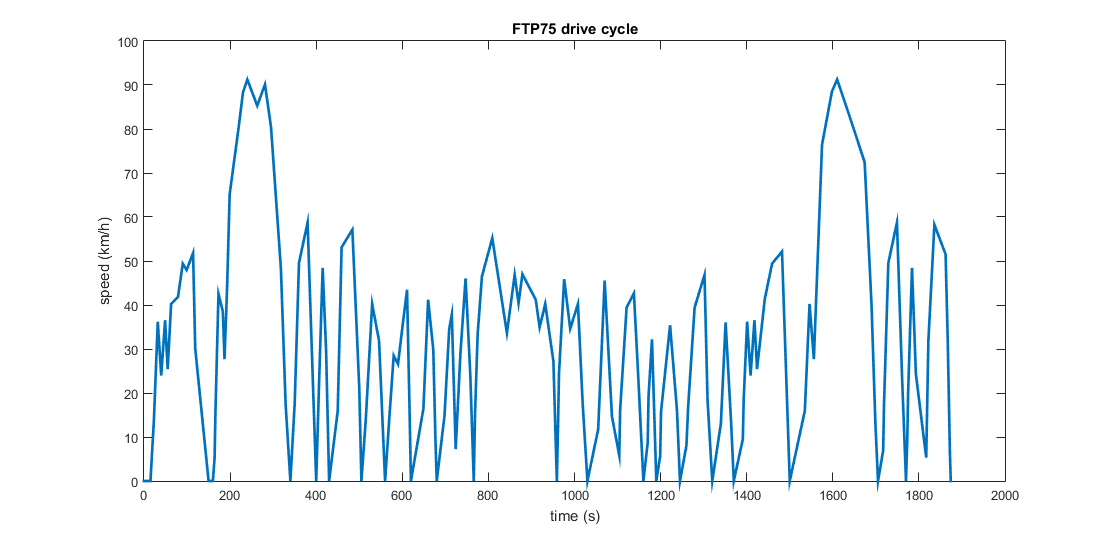
\includegraphics[scale=0.45]{figures/FTP75}
\caption{FTP drive cycle}
\label{fig:ftp75}
\end{figure}

The NEDC drive cycle was invented to test light-duty cars in Europe. Its duration is 1180s, the distance is 11.02km and the average speed 33.6km/h. It contains four equivalent urban driving phases called ECE-15. They last from 0-780s and there is also a fourth highway driving phase called EUDC from 781-1180s. Figure \ref{fig:nedc} shows the time versus the speed in the NEDC drive cycle.

\begin{figure}[h]
\centering
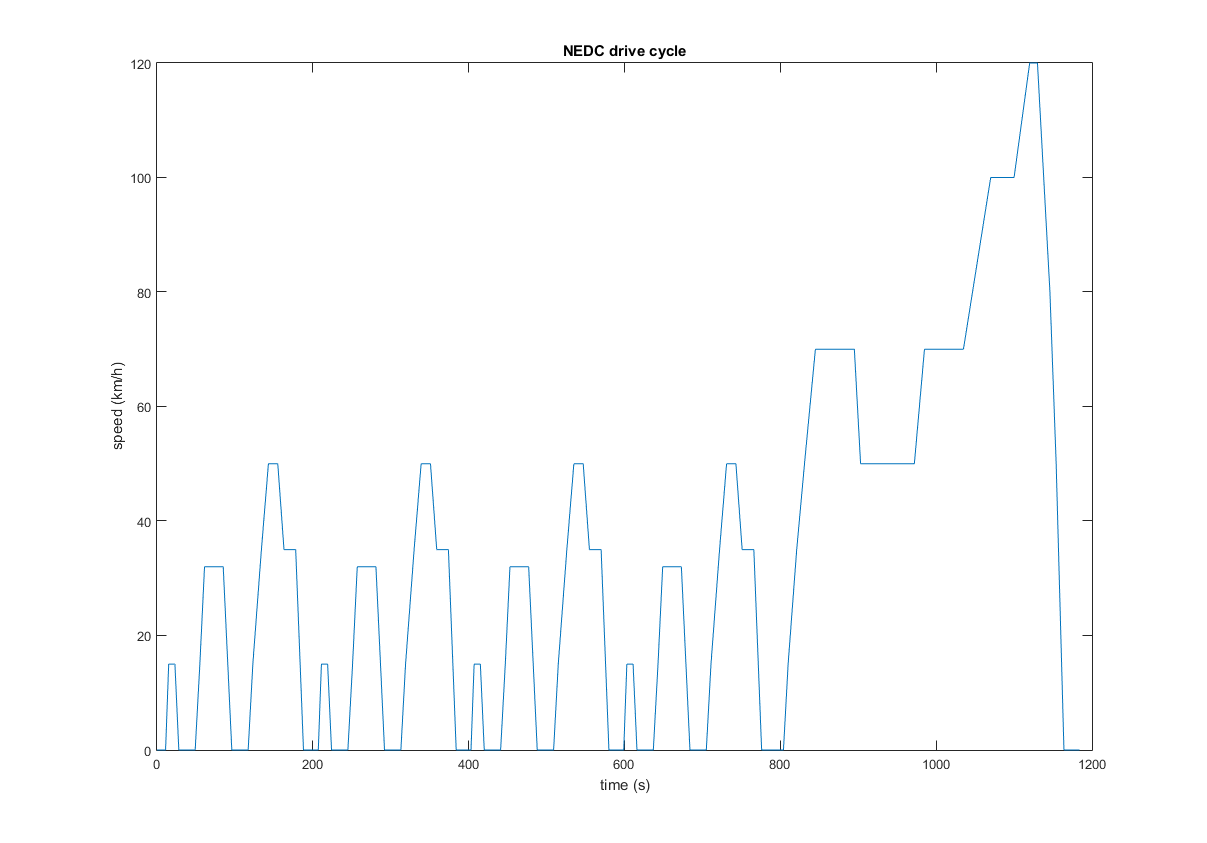
\includegraphics[scale=0.45]{figures/NEDC}
\caption{NEDC drive cycle}
\label{fig:nedc}
\end{figure}

The Speed Control block takes as input the demanded speed from the drive cycle and the actual speed of the vehicle both in \textit{km/h} and calculates as output the acceleration which lies between -1 and 1 where a negative value means braking and a positive value means acceleration. A value of 0 corresponds to cruising or maintaining a constant speed. In order to calculate the acceleration demand, the difference between the demanded and actual speed is taken.

\subsection{Power Controller}
The Power Controller takes as input the acceleration demand $a$ and the state of charge $SOC$ of the battery which comes from the Electric Motor Controller. In order to transform the acceleration demand into torque demand $\tau_{dem}$, the acceleration is scaled by the maximum torque of 400 \textit{Nm} which can be requested. This value was chosen since this is the maximum output torque of the Toyota Prius electric motor. The minimum demanded torque is -400 \textit{Nm} which corresponds to deceleration. The current motor speed $\omega_{eng}$ is mapped to the torque of the motor which it is capable of generating at this moment. This value is taken as upper limit and its negated value is taken as a lower limit of the torque. 

There are two subsystems in the Power Controller, the Battery Management and the Game Theory Controller. The first of them takes as input the battery $SOC$, its current in \textit{A}, its voltage in \textit{V} and computes the required recharge power $P_{batReq}$ and the battery limit $P_{batLim}$. The recharge power is requested when the SOC of the battery lies between 40 and 60\%. If the SOC falls below 40\% then the battery is forced to be recharged even if that means not meeting the drive cycle requirements and the demanded speed cannot be achieved. After the battery has been charged up to 60\%, the recharging stops and the required battery power is set to 0. The battery limit calculation takes into account that the maximum voltage of the battery is 200V and that its maximum power is 21 kW.

The Game Theory Controller is the primary place where the computation of the solution to the power distribution problem happens. The outputted demanded torque $\tau_{dem}$ is fed into the Game Theory Controller block. In addition, the other inputs of this block are required power, which is:
\begin{equation}
P = \tau \times \omega
\end{equation}
where power $P$ is in \textit{W}, torque $\tau$ is in \textit{Nm} and the velocity $\omega$ is angular \textit{rad/s}.
The Game Theory Controller also receives the battery SOC in \%, the generator $\omega_{gen}$, engine $\omega_{eng}$, motor $\omega_{mot}$ speeds all in \textit{rad/s}, the Total Fuel consumed up to this moment from the beginning of the drive cycle $TF$ in \textit{litres}, the battery limit and the required battery recharge power $P_{batReq}$ as described in the Battery Management subsystem above. The Game Theory Controller block contains the game-theoretical logic embedded as a Matlab function. Apart from it, it also regulates the speed of the engine by taking the difference between the required driving power $P_{drive}$ and the recharge power for the battery $P_{batReq}$. The resulting power is given as an input to a lookup table to find the corresponding engine speed in \textit{rpm}. To obtain the Generator torque $\tau_{gen}$ the engine torque and the generator speed $\omega_{gen}$ in \textit{rad/s} are taken. If the motor needs to provide additional power for the battery, this power is taken to be the sum of the battery available power and the generator power. The battery available power $P_{batAv}$ is computed in a separate subsystem using the engine torque $tau_{end}$, speed $\omega_{eng}$ and power $P_{eng}$, battery recharge power $P_{batReq}$ and battery limit $P_{batLim}$. 
As a result from the Game Theory Controller the engine throttle $\theta$, the motor torque $\tau_{mot}$, the generator torque $\tau_{gen}$, the reference engine speed in \textit{rpm} $\omega_{eng}$. These are fed to a final Speed Controller block for controlling the engine speed which outputs the final engine throttle $\theta$ as percentage from the maximum possible torque of the engine $\tau_{engMax}$.

\section{Game-theoretical algorithms}
This chapter describes the implementation of all six game-theoretical approaches in Matlab.